\graphicspath{{images/}}

\section{Численные методы решения дифференциальных уравнений с частными производными}

\subsection{Численные методы решения ДУЧП параболического типа}

\subsubsection{Постановка задачи}
Используя явную и неявную конечно-разностные схемы, а также схему Кранка-Николсона, решить начально-краевую задачу для дифференциального уравнения параболического типа. Осуществить реализацию трёх вариантов аппроксимации граничных условий, содержащих производные: двухточечная аппроксимация с первым порядком, трёхточечная аппроксимация со вторым порядком, двухточечная аппроксимация со вторым порядком. В различные моменты времени вычислить погрешность численного решения путем сравнения результатов с приведенным в задании аналитическим решением $U(x, t)$. Исследовать зависимость погрешности от сеточных параметров $\tau$, $h$.

\subsubsection{Вариант 10}
$$ {{\partial u} \over {\partial t}} = a \cdot {{\partial^2 u} \over {\partial x^2}} + b \cdot {{\partial u} \over {\partial y}} + c \cdot u $$
$$ a > 0, b > 0, c < 0 $$
$$ u'_x(0, t) + u(0, t) = e ^ {(c - a) t} \cdot (\cos(bt) + \sin(bt)) $$
$$ u'_x(\pi, t) + u(\pi, t) = -e ^ {(c - a) t} \cdot (\cos(bt) + \sin(bt)) $$
$$ u(x, 0) = \sin{x} $$
Аналитическое решение:
$$ U(x, t) = e ^ {(c - a) t} \cdot \sin(x + bt) $$
\pagebreak

\subsubsection{Результат}
\begin{center}
    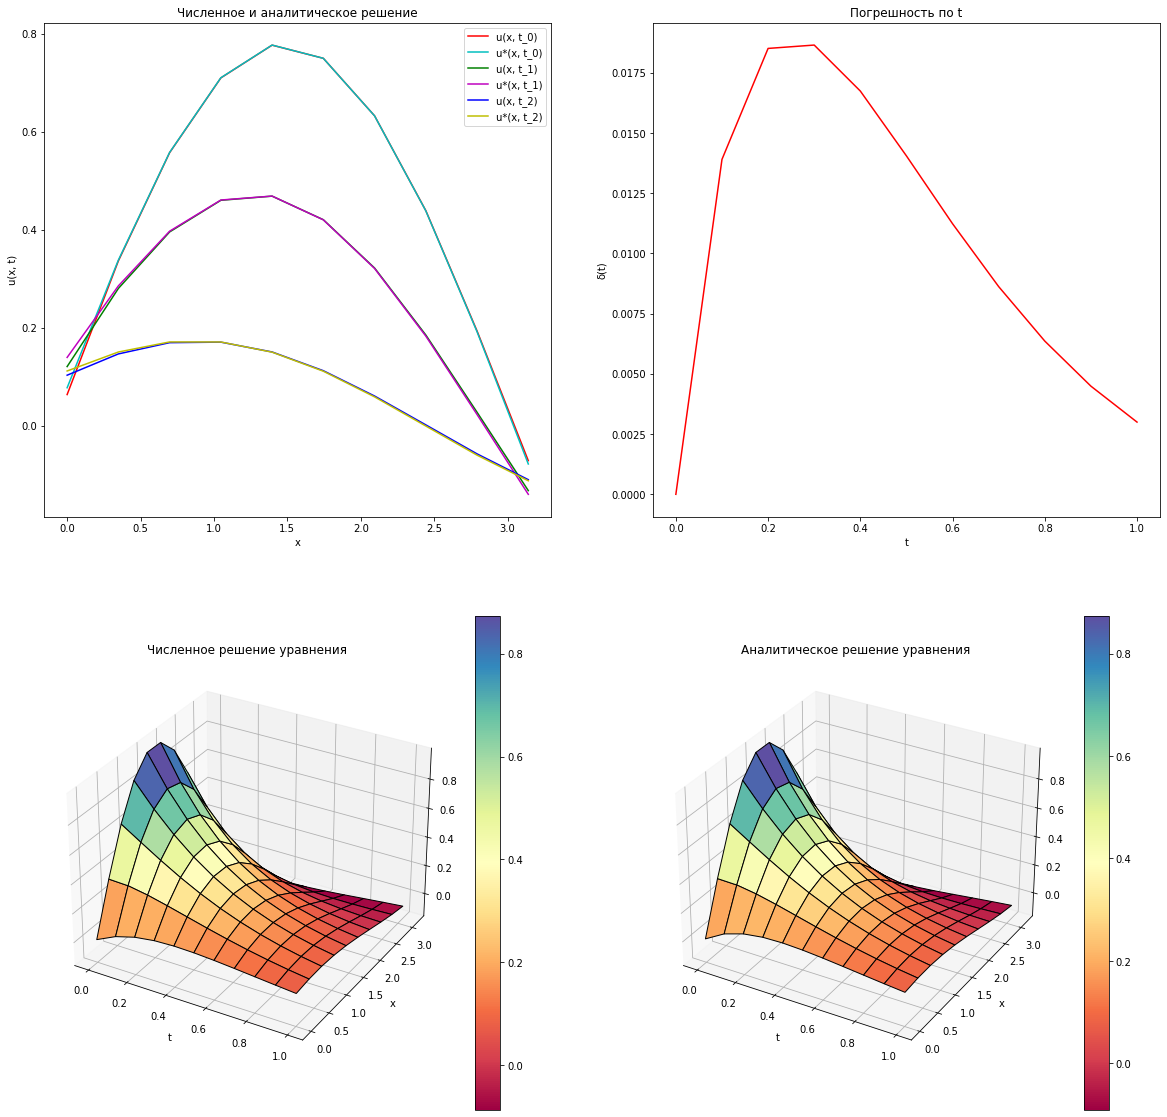
\includegraphics[width=\textwidth]{5.png}\newline\noindent
\end{center}
\pagebreak

\subsubsection{Исходный код}
\lstinputlisting{../lab5/ppde.hpp}
\pagebreak
